\documentclass[11pt,a4paper,titlepage]{article}
\usepackage[utf8]{inputenc}
\usepackage[margin=2cm,headheight=13.6cm]{geometry}
\usepackage{color}
% Agregados por mi
\usepackage{empheq}
\newcommand*\widefbox[1]{\fbox{\hspace{2em}#1\hspace{2em}}}
\usepackage{ifpdf}
\usepackage{hyperref}
\usepackage{booktabs}
\usepackage{amsmath}
\usepackage{mathtools}
\usepackage{amsfonts}
\usepackage{enumerate}
\usepackage{verbatim}
\usepackage{tikz}
\usetikzlibrary{shapes,snakes}
\newcommand*{\TitleParbox}[1]{\parbox[c]{3.75cm}{#1}}%
\newcommand*{\ntpb}[1]{\parbox[c]{3cm}{#1}}%
\usepackage{multicol}
\usepackage{cancel}
% Command "alignedbox{}{}" for a box within an align environment
% Source: http://www.latex-community.org/forum/viewtopic.php?f=46&t=8144
\newlength\dlf  % Define a new measure, dlf
\newcommand\alignedbox[2]{
% Argument #1 = before & if there were no box (lhs)
% Argument #2 = after & if there were no box (rhs)
&  % Alignment sign of the line
{
\settowidth\dlf{$\displaystyle #1$}  
    % The width of \dlf is the width of the lhs, with a displaystyle font
\addtolength\dlf{\fboxsep+\fboxrule}  
    % Add to it the distance to the box, and the width of the line of the box
\hspace{-\dlf}  
    % Move everything dlf units to the left, so that & #1 #2 is aligned under #1 & #2
\boxed{#1 #2}
    % Put a box around lhs and rhs
}
}

%Para el underbracket con el igual
\newlength\diz  % Define a new measure, diz
\newcommand\alignedunderbracket[2]{
% Argument #1 = before & if there were no box (lhs)
% Argument #2 = after & if there were no box (rhs)
&  % Alignment sign of the line
{
\settowidth\diz{$\displaystyle #1$}  
    % The width of \diz is the width of the lhs, with a displaystyle font
\addtolength\diz{\fboxsep+\fboxrule}  
    % Add to it the distance to the box, and the width of the line of the box
\hspace{-\diz}  
    % Move everything diz units to the left, so that & #1 #2 is aligned under #1 & #2
\underbracket{#1 #2}
    % Put a box around lhs and rhs
}
}

%Fin de agregados por mi
\usepackage{listings}
\usepackage{graphicx}
\usepackage[spanish]{babel}
\usepackage{caption}
\usepackage{subcaption}
\usepackage{float}
\usepackage{titling}
\usepackage{pgfkeys}
\definecolor{mygreen}{RGB}{0,127,0}
\definecolor{mygray}{RGB}{100,100,100}
\definecolor{mymauve}{RGB}{100,32,255}
\definecolor{lgray}{RGB}{230,230,230}
\lstset{ %
  frame=none,
  backgroundcolor=\color{white},   % choose the background color; you must add \usepackage{color} or \usepackage{xcolor}
  basicstyle=\footnotesize\ttfamily,        % the size of the fonts that are used for the code
  breakatwhitespace=false,         % sets if automatic breaks should only happen at whitespace
  breaklines=true,                 % sets automatic line breaking
  captionpos=t,                    % sets the caption-position to bottom
  commentstyle=\color{mygreen},    % comment style
  deletekeywords={...},            % if you want to delete keywords from the given language
  escapeinside={\%*}{*)},          % if you want to add LaTeX within your code
  extendedchars=true,              % lets you use non-ASCII characters; for 8-bits encodings only, does not work with UTF-8
%  frame=single,                    % adds a frame around the code
  keepspaces=true,                 % keeps spaces in text, useful for keeping indentation of code (possibly needs columns=flexible)
  keywordstyle=\color{blue},       % keyword style
  language=,                 % the language of the code
  morekeywords={*,...},            % if you want to add more keywords to the set
  numbers=left,                    % where to put the line-numbers; possible values are (none, left, right)
  numbersep=5pt,                   % how far the line-numbers are from the code
  numberstyle=\tiny\color{mygray}, % the style that is used for the line-numbers
  rulecolor=\color{black},         % if not set, the frame-color may be changed on line-breaks within not-black text (e.g. comments (green here))
  showspaces=false,                % show spaces everywhere adding particular underscores; it overrides 'showstringspaces'
  showstringspaces=false,          % underline spaces within strings only
  showtabs=false,                  % show tabs within strings adding particular underscores
  stepnumber=1,                    % the step between two line-numbers. If it's 1, each line will be numbered
  stringstyle=\color{mymauve},     % string literal style
  tabsize=4,                       % sets default tabsize to 2 spaces
  aboveskip=3mm,
  belowskip=3mm,
}

\usepackage{fancyhdr}
\pagestyle{fancy}
\rhead{}
\usepackage{datetime}
\usepackage{moresize}

\newdateformat{monthyeardate}{%
  \monthname[\THEMONTH] \THEYEAR}

\newcommand{\rulebreak}{%
	\par%
	\vspace{0.9cm}%
    \noindent\rule{4cm}{0.4pt}%
    \vspace{1.2cm}%
    \par%
}

\newcommand{\coverpage}[1]{%
	\pagenumbering{roman}%
	\thispagestyle{empty}%
	\lhead{\textsc{\small{TP 1:} #1}}%
    \title{Diseño Analógico de Circuitos Integrados}%
    \author{Autor: Leandro Marsó,
    \\
            Profesores: Benjamín Reyes}%
    \newgeometry{left=5cm,bottom=2cm,right=5cm,top=2cm}%
	\begin{center}\hspace{0pt}\vfill%
    \uppercase{
    Universidad Nacional de Córdoba\\
    Facultad de Ciencias Exactas, Físicas y Naturales
    }
	\rulebreak%
    {\Large\textbf{Diseño Analógico de Circuitos Integrados}}
    
    \vspace{0.5cm}
    {\HUGE\textbf{\textit{#1}}}
    
    \vspace{0.5cm}
	\theauthor%
	\par%
	\vspace{0.9cm}%
    \noindent\rule{4cm}{0.4pt}%
    \vspace{0.45cm}
    \tableofcontents%
	\rulebreak%
    \monthyeardate\today\par
    \hspace{0pt}
	\end{center}%
    \vfill
    \hspace{0pt}
	\pagebreak%
    \restoregeometry%
    \pagenumbering{arabic}%
}

% Custom arguments for /fig command
\pgfkeys{
 /fig/.is family, /fig,
 default/.style = 
  {scale = 1,
   angle = 0},
 scale/.estore in = \figScale,
 angle/.estore in = \figAngle
}
\newcommand{\fig}[2][]{%
	\pgfkeys{/fig, default, #1}%
	\begin{figure}[H]%
    \centering
    \includegraphics[angle=\figAngle,width=\figScale\textwidth]{#2}%
	\end{figure}%
}

\newcommand{\filename}[1]{%
	\texttt{#1}%
}

\newcommand{\vhdl}[1]{%
  \lstinputlisting[language=vhdl]{#1}
}

\newcommand*\paths[1]{\lstset{inputpath=#1}\graphicspath{#1}}


\everymath{\displaystyle} %Esto es para que la matemática dentro de texto sea más grande que el texto

\begin{document}
\coverpage{TP 1}
  
\subsection{Canal Corto vs. Canal largo}
Comparación de curvas del NMOS para canal largo y canal corto. El transistor M1 es de canal corto ($L_1=0.6\mu m$), M2 tiene $L_2=3\mu m$ y $L_3=6\mu m$.
\subsubsection{$I_D$ vs. $V_{GS}$}
\vspace{0.3cm}
\begin{figure}
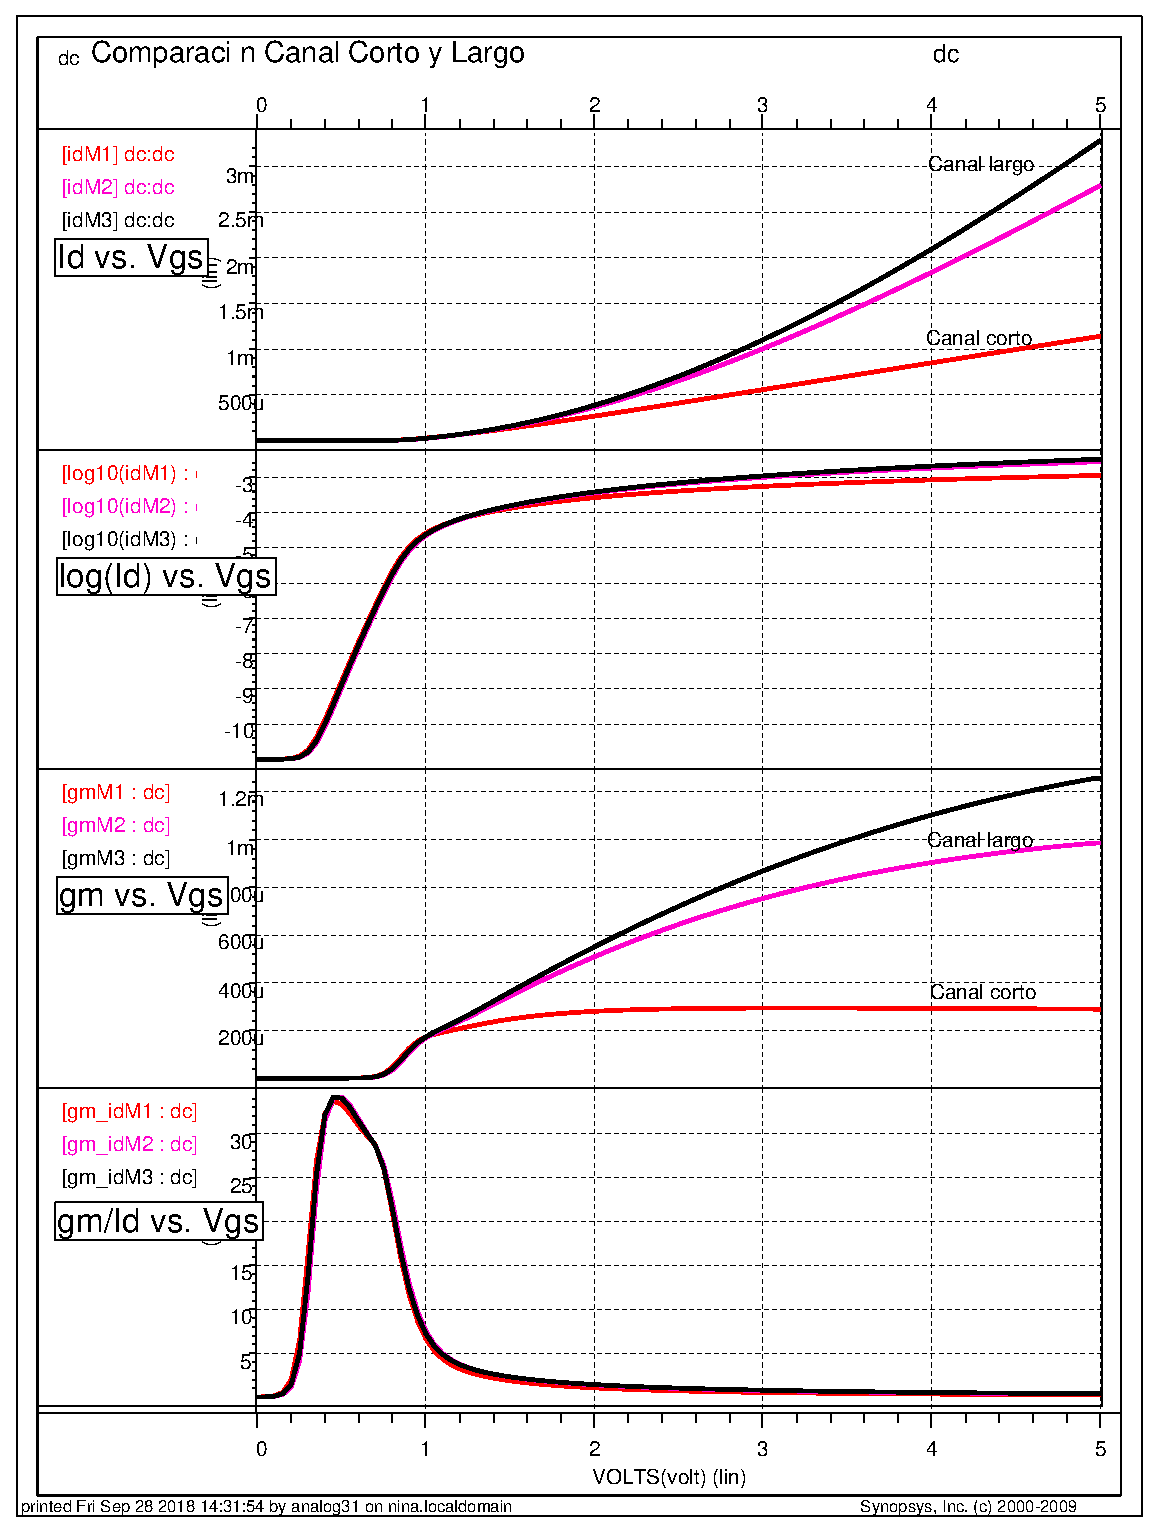
\includegraphics[scale=0.6, angle=0]{images/todas}
\captionof{figure}{$I_D$, $\log(I_D)$, $g_m$, $\frac{g_m}{I_D}$ vs. $V_{GS}$ (escala lineal)}
\label{fig:ids_vgs}
\end{figure}
De las simulaciones dc y op obtenemos las curvas de la figura \ref{fig:ids_vgs} y los siguientes $V_{th}$ para cada transistor:

%\subsubsection{$I_D$ vs. $V_{GS}$} 
\begin{itemize}
	\item $V_{th}$ de M1 ($L=0.6\mu$m): $0.674243$V
	\item $V_{th}$ de M2 ($L=3\mu$m): $0.69121$V
	\item $V_{th}$ de M3 ($L=6\mu$m): $0.680835$V
\end{itemize}

\paragraph{Ley Cuadrática}

Observando la primera curva de la figura \ref{fig:ids_vgs} ($I_D$ vs. $V_{GS}$) vemos una relación cuadrática a partir de $V_{TH}$ entre la tensión de compuerta y la corriente de drenador. Para canal corto se nota menos pronunciada está relación, debido a que en este caso el \emph{pinch-off} se dá lejos del drenador. Otra razón es la degradación de la movilidad de los portadores. En resumen, tienen mucha influencia los efectos de segundo orden que se desprecian para obtener la función cuadrática. 

\paragraph{Variación de la tensión de \emph{threshold}}
Al mismo tiempo, vemos que el $V_{th}$ del transistor de canal corto tiene un valor menor que M2 y M3, esto es debido principalmente a que el drain y source también aportan a generar carga inmóbil en el canal debido a lo corto del canal, y el gate necesita menor tensión para llegar a la invertir el canal. 

El $V_{th}$ de M3 es menor al de M2 debido al efecto reverso de canal corto (\emph{reverse short-channel effect}), que determina que a medida que crece el largo del canal, decrece el $V_{th}$.

\paragraph{Saturación de velocidad}
Este efecto se da cuando el campo eléctrico lateral formado por la diferencia de potencial entre drenador y surtidor supera cierto valor (1V/$\mu$m) y la movilidad de los portadores comienza a decaer. Podemos ver saturación de velocidad en el transistor de canal corto cuando el incremento de corriente en las curvas paramétricas (Id vs. Vds figura \ref{fig:parametric} ) es constante. Más notable es este efecto en la curva $g_m$ vs. $v_{gs}$ que es prácticamente constante el valor de $g_m$ en la zona de inversión fuerte. También ya hemos resaltado este efecto en la curva $I_d$ vs. $V_{gs}$ en M1.

\subsubsection{$\log{(I_D)}$ vs. $V_{GS}$} 

\paragraph{Corrientes sub-umbral}
Podemos ver en la figura \ref{fig:ids_vgs} (en el segundo conjunto de curvas), que los tres transistores en la zona de subumbral tienen el mismo comportamiento.


\subsubsection{$I_D$ vs. $V_{GS}$}
\begin{figure}
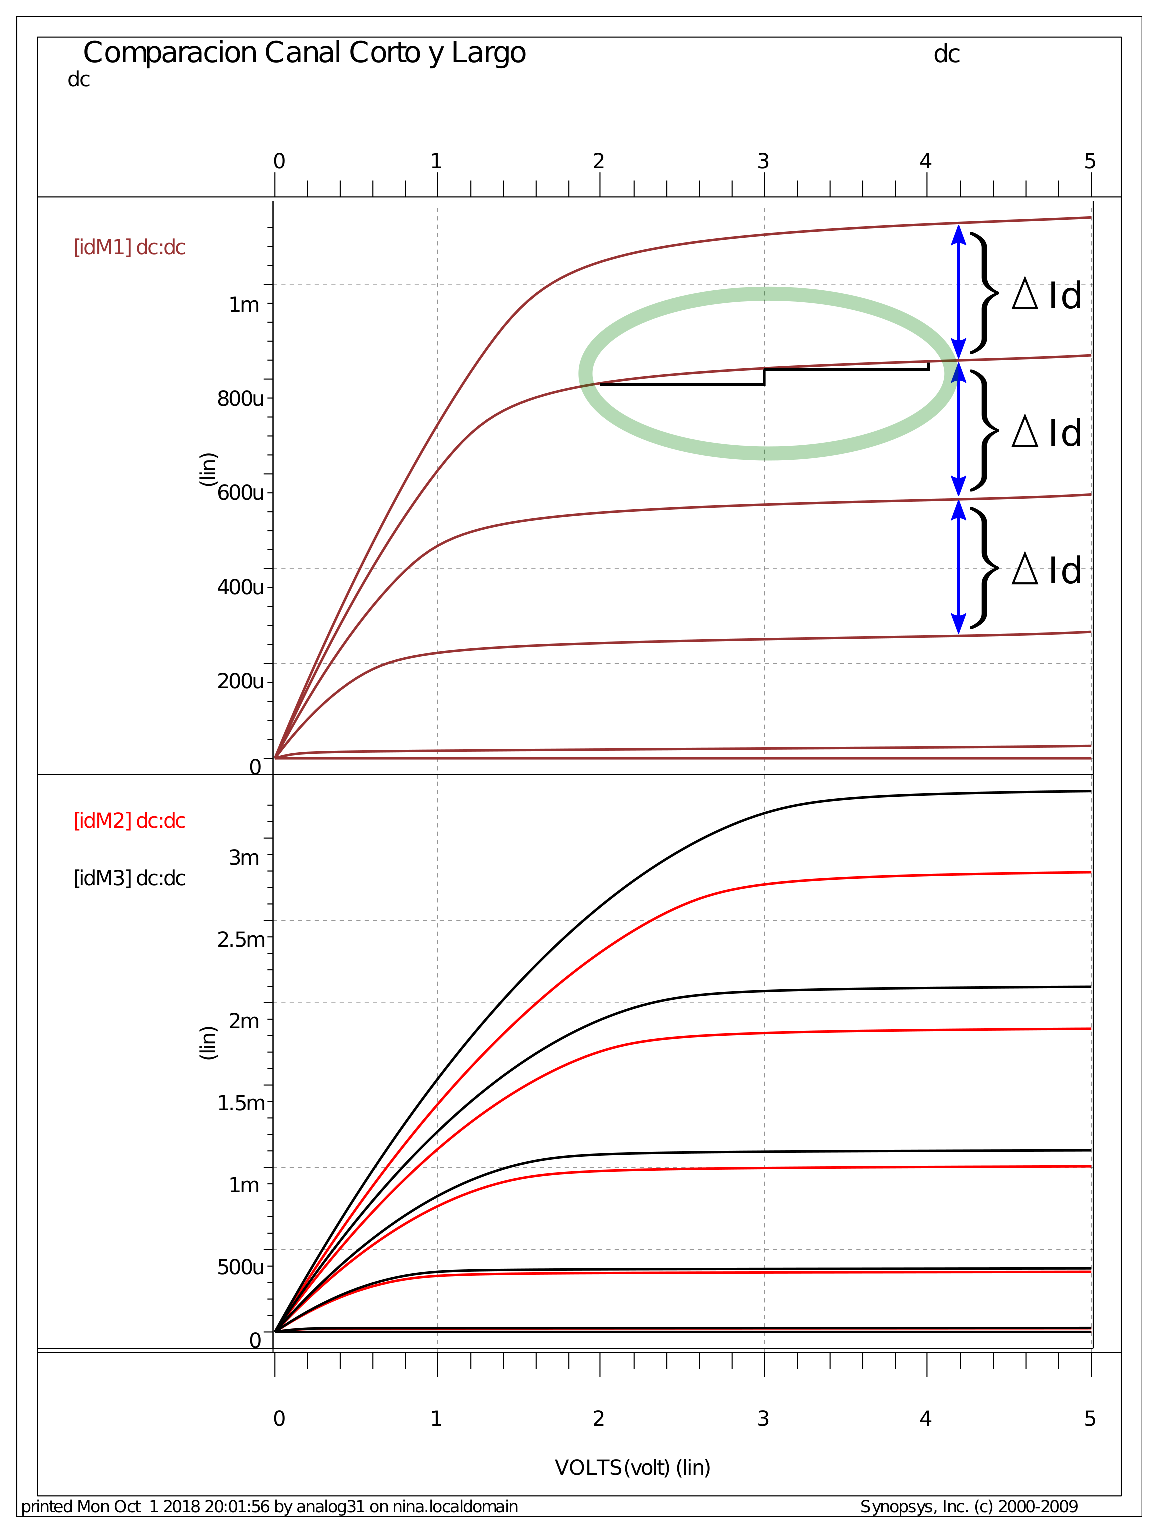
\includegraphics[scale=0.56]{images/parametric}
\captionof{figure}{$I_D$ vs. $V_{DS}$ , barriendo $V_{GS}$ de forma paramétrica}
	\label{fig:parametric}
\end{figure}
%Evaluando la curva I D vs. V DS con barrido paramétrico de V GS , SAE Fig:3:
%• Comparar cómo varía λ para los distintos niveles de I D (cambios en la pendiente de
%corriente en saturación).
\paragraph{Pendiente en la corriente de saturación}
Se puede notar cómo aumenta la pendiente según aumenta la $V_{gs}$ para los tres transistores.

Pero en el de canal corto esta pendiente siempre es bastante más pronunciada
%• Comparar cómo varía λ para canal corto y canal largo.
%• Comparar cómo varía I D para un mismo V GS entre canal corto y canal largo.

\begin{figure}[!tbp]
   \begin{subfigure}[b]{0.3\textwidth}
       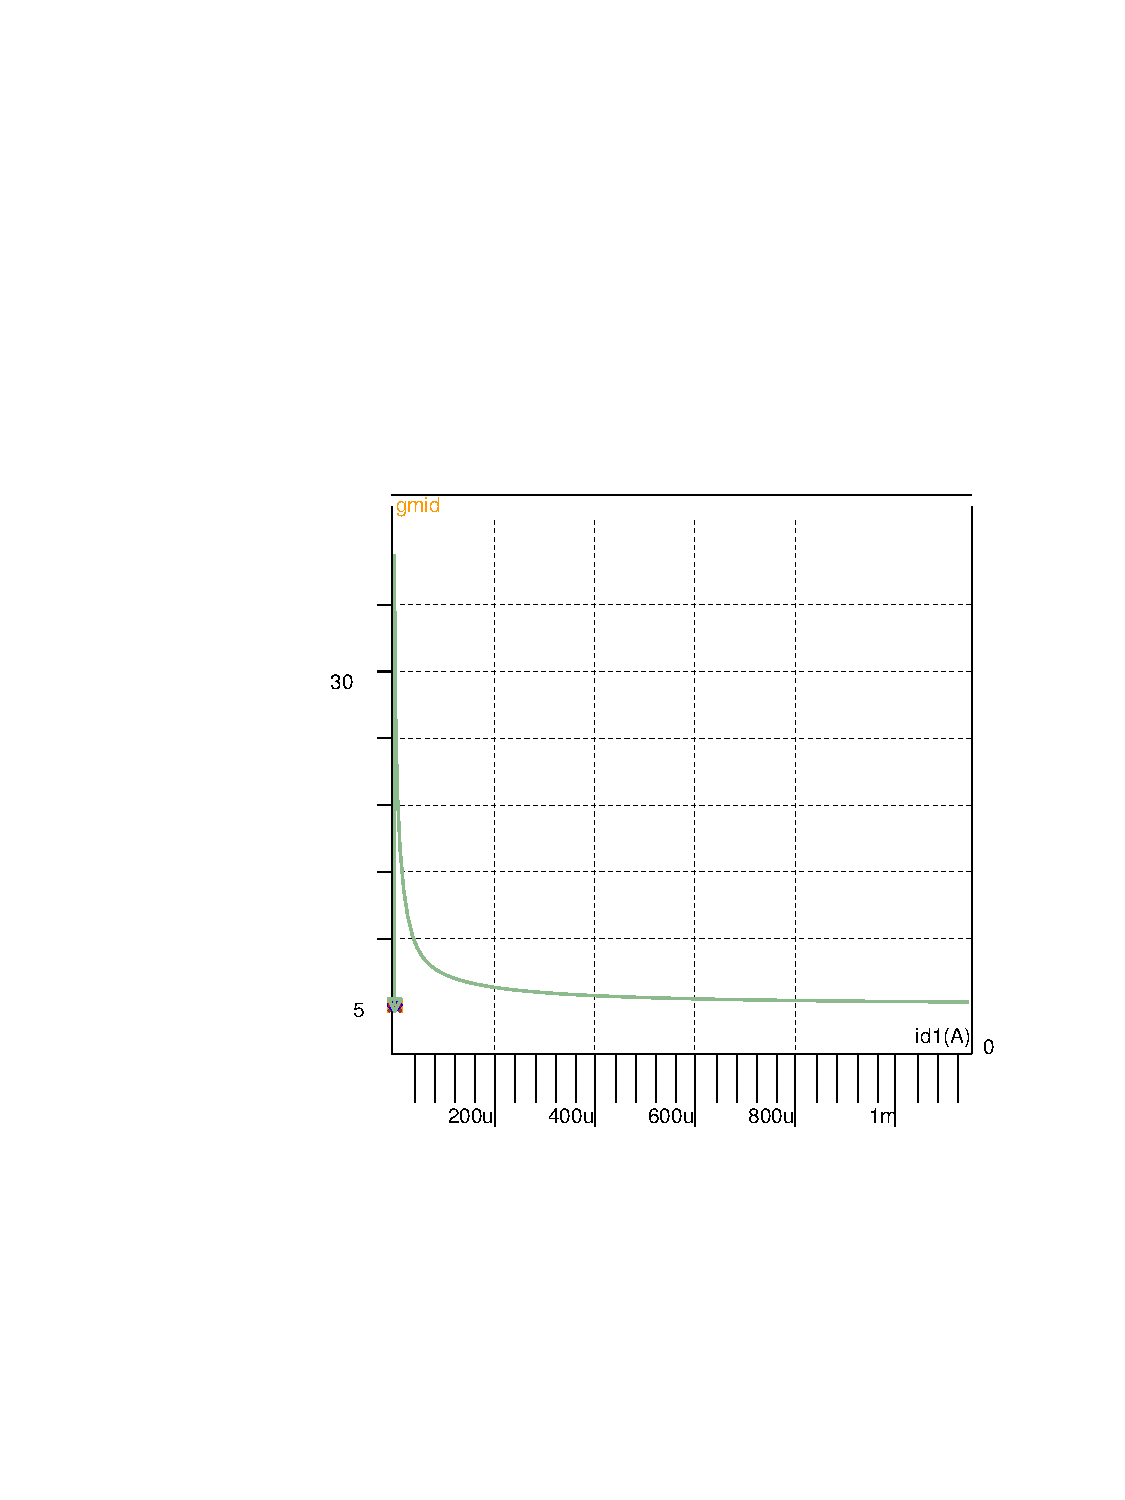
\includegraphics[width=\textwidth]{images/gmid_id_m1}
   \caption{M1}
   \label{fig:f1}
   \end{subfigure}
   \begin{subfigure}[b]{0.34\textwidth}
   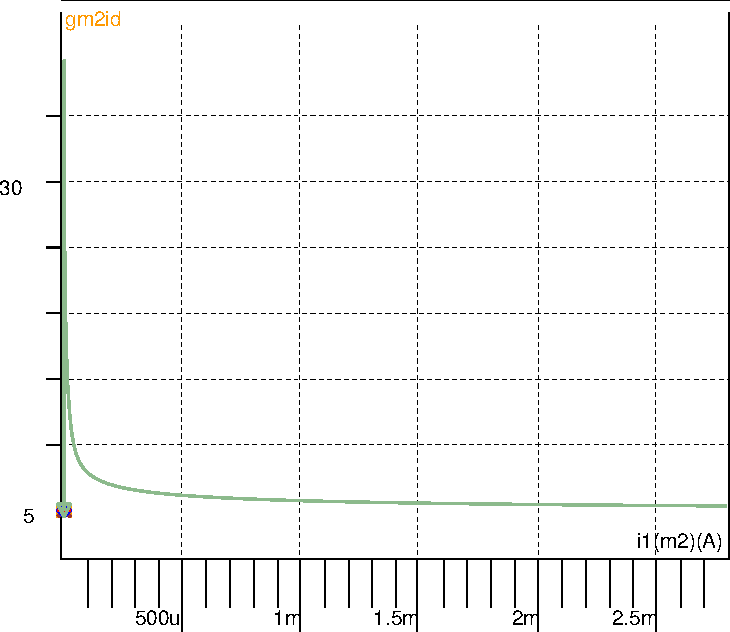
\includegraphics[width=\textwidth]{images/gmid_id_m2}
   \caption{M2}
   \label{fig:f2}
   \end{subfigure}
 \begin{subfigure}[b]{0.34\textwidth}
   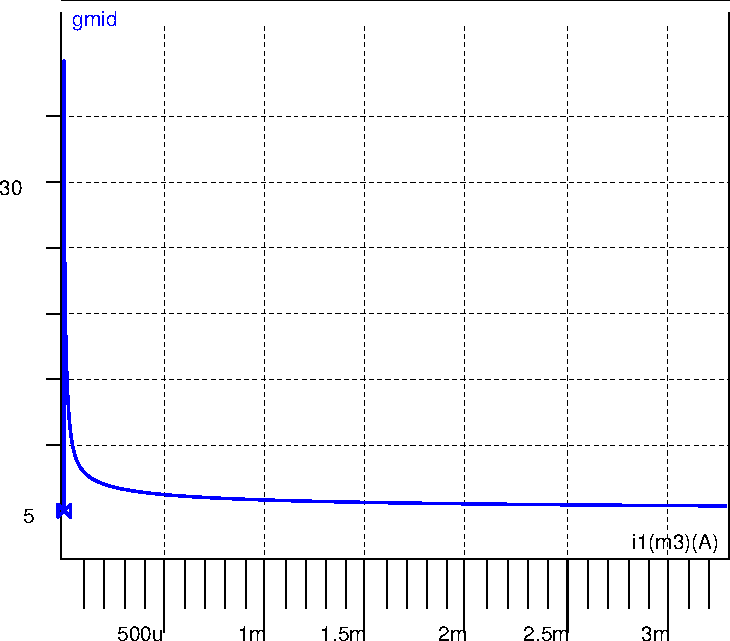
\includegraphics[width=\textwidth]{images/gmid_id_m3}
   \caption{M3}
   \label{fig:f3}
   \end{subfigure}
    %\caption{gm/id Vs. id}
    \caption{$\frac{g_m}{I_d}$ vs. $I_d$}

\end{figure}

\begin{figure}[!tbp]
   \begin{subfigure}[b]{0.25\textwidth}
       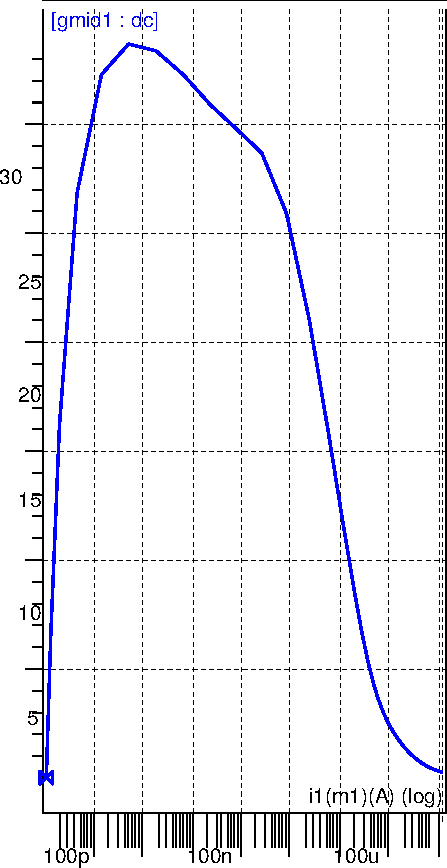
\includegraphics[width=\textwidth]{images/gmid_log10id_m1}
   \caption{M1}
   \label{fig:f1}
   \end{subfigure}
 %  \hfill
   \begin{subfigure}[b]{0.35\textwidth}
   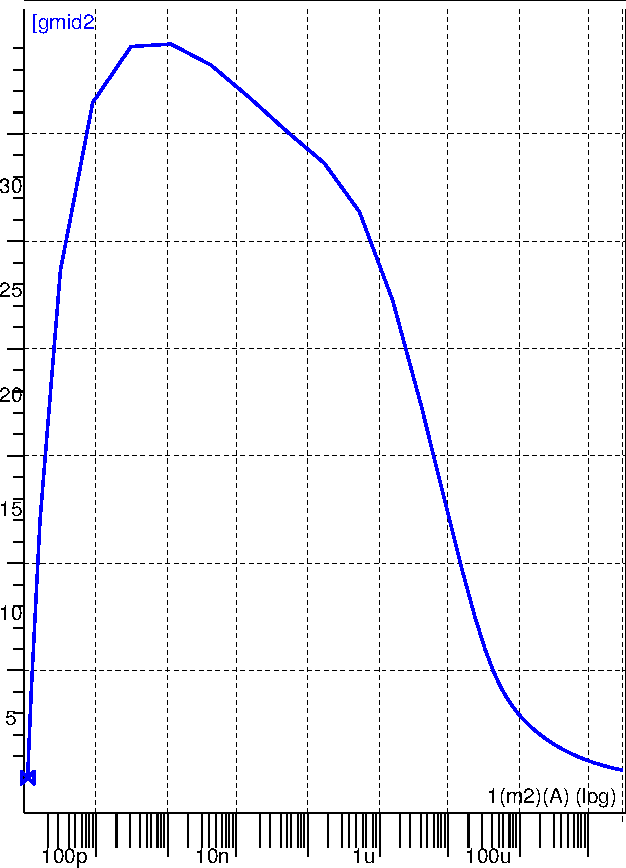
\includegraphics[width=\textwidth]{images/gmid_log10id_m2}
   \caption{M2.}
   \end{subfigure}
 \begin{subfigure}[b]{0.355\textwidth}
   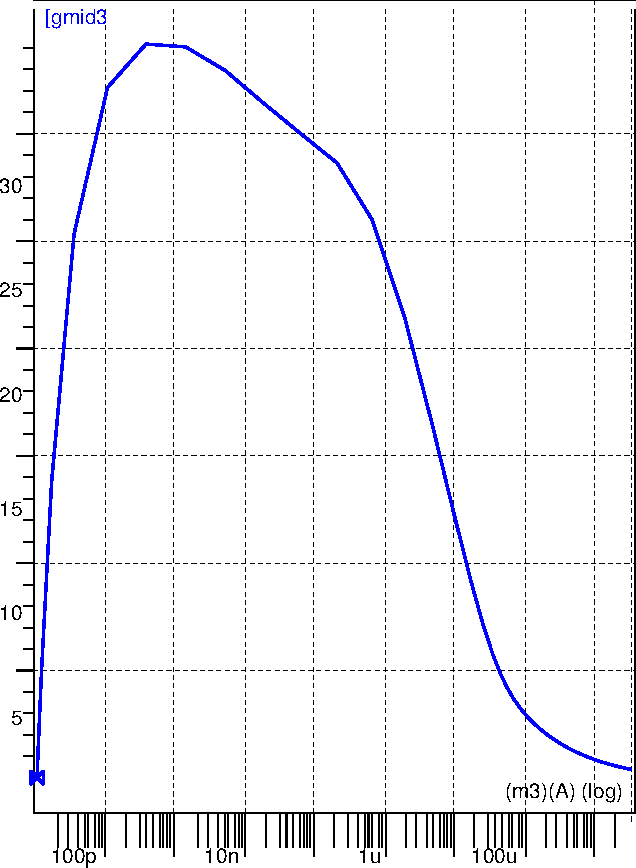
\includegraphics[width=\textwidth]{images/gmid_log10id_m3}
   \caption{M3.}
   \label{fig:f2}
   \end{subfigure}
    \caption{$\frac{g_m}{I_d}$ vs. $\log_{10}(I_d)$}
\end{figure}



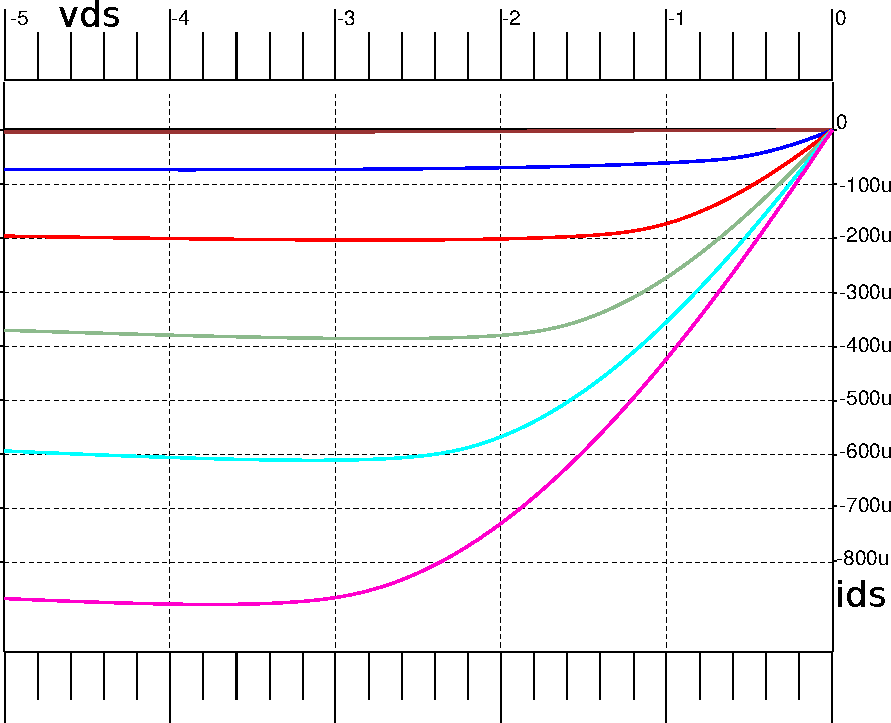
\includegraphics[scale=0.8]{images/pmos_vgs_param}
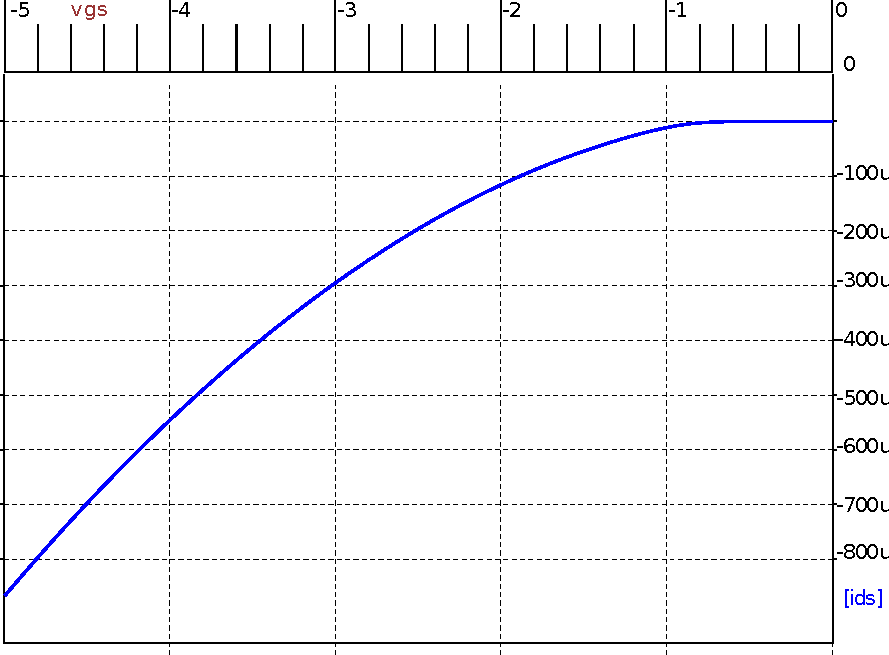
\includegraphics[scale=0.8]{images/pmos_vds_vgs}
%%%\captionof{figure}{bla}

%\vspace{1cm}

%\subsubsection*{Ejercicio 2}
\end{document}
